%*****************************************************************
\section{Gaussian Process Fundamentals}\label{sec:gp_fundamentals}
%*****************************************************************

This section reviews the basics of \gls[hyper=false]{gp}.
The connection between the stochastic process and multivariate Gaussian random variable (Gaussian random vector) is first established.
Appendix~\ref{app:probability} gives some basic concepts of multivariate random variable such as joint, marginal, and conditional probabilities, 
while Appendix~\ref{app:gaussian_vector} gives more detail account on Gaussian random vector (\gls[hyper=false]{mvn}).

\subsection[From Multivariate Gaussian to Gaussian Process]{From Multivariate Gaussian to Gaussian Process}\label{sub:gp_mvn}

% Illustration of Joint, Marginal, and Conditional
To illustrate the notions of joint, marginal, and conditional distributions, an example of a bivariate random variable, a random vector $\bm{\mathcal{Z}} = [\mathcal{Z}_1, \mathcal{Z}_2] \in \mathbb{R}^2$ is given.
\marginpar{random vector, an example}
It has the following mean vector and variance-covariance matrix, respectively,
\begin{equation}
	\begin{split}
		\begin{pmatrix}
			\mathcal{Z}_1 \\
			\mathcal{Z}_2
		\end{pmatrix} & \sim \mathcal{N}(\boldsymbol{\mu}, \boldsymbol{\Sigma}) \\
		 \boldsymbol{\mu} & = [0, 0]^T \\
		  \boldsymbol{\Sigma} = 
				\begin{pmatrix}
					\mathbb{V}[\mathcal{Z}_1]                 & \text{Cov}[\mathcal{Z}_1, \mathcal{Z}_2]\\
					\text{Cov}[\mathcal{Z}_2, \mathcal{Z}_1]  & \mathbb{V}[\mathcal{Z}_2]\\
			\end{pmatrix} & =
			\begin{pmatrix}
					0.5       & -0.265165\\
					-0.265165 & 0.25\\
			\end{pmatrix}
	\end{split}
\label{eq:ex_bivariate}
\end{equation}
The joint, marginal, and conditional \glspl[hyper=false]{pdf} of random vector $\bm{\mathcal{Z}}$ are illustrated in Fig.~\ref{fig:plot_bivariate_normal}.
\begin{figure}[bth]
	\centering
	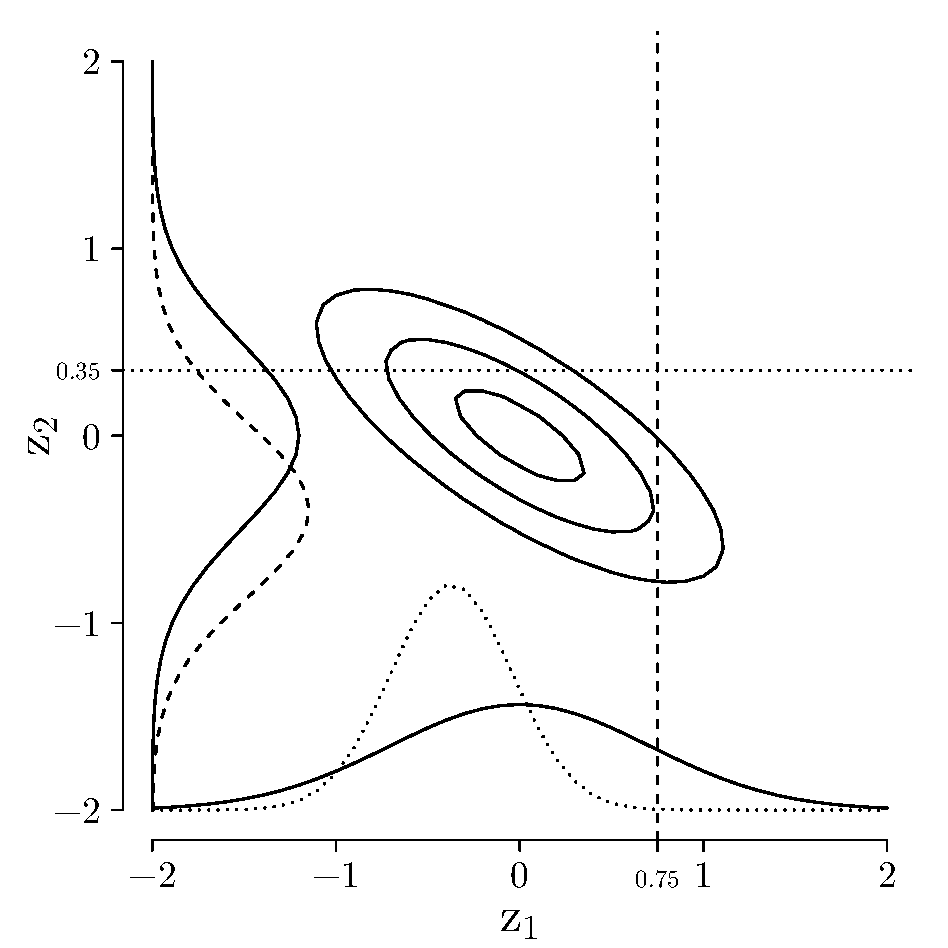
\includegraphics[scale=0.50]{../figures/chapter4/figures/plotBivariateNormal.pdf}
	\caption[Illustration of a bivariate Gaussian distribution]{An illustration of bivariate Gaussian distribution of random vector $\bm{\mathcal{Z}} = [\mathcal{Z}_1, \mathcal{Z}_2] \in \mathbb{R}^2$ having marginal means of $0.0$ and variances of $0.5$ and $0.25$, respectively and with covariance of $-0.265165$. The solid ellipsoids indicate the contour of joint \gls[hyper=false]{pdf} of random vector $[\mathcal{Z}_1, \mathcal{Z}_2]$. The two solid curves at the $x$- and $y$-axes indicate the marginal \gls[hyper=false]{pdf} of $\mathcal{Z}_1$ and $\mathcal{Z}_2$, respectively. The dotted curve shows the conditional density of random variable $\mathcal{Z}_1$ given $z_2 = 0.35$, while the dashed curve shows the conditional density of $\mathcal{Z}_2$ given $z_1 = 0.75$.}
	\label{fig:plot_bivariate_normal}
\end{figure}

The joint density for Gaussian random vector is given in Eq.~(\ref{eq:gaussian_joint_density}.
\marginpar{joint density, illustrated}
For the bivariate random variable in the example, the density can be shown as contour plot in Fig.~\ref{fig:plot_bivariate_normal}.
In the figure, the solid ellipsoids are the iso-contours of the distribution, where each pair of values lies along the contour line has the same probability density value.

The two marginal densities for the example are shown as the solid curves plotted in the $x$ and $y$-axes, respectively.
\marginpar{marginal density, illustrated}
As illustrated, the marginalization of the joint distribution can be thought as a \emph{projection} of the $2$-dimensional distribution into each of the corresponding dimension.

Finally, two conditional distributions $p(z_1|z_2=0.35)$ and $p(z_2|z_1=0.75)$ are given as examples of conditioning a probability distribution in Fig.~\ref{fig:plot_bivariate_normal}.
\marginpar{conditional density, illustrated}
They are shown as dotted and dashed curves plotted in both axes.
Conditioning can be thought of as \emph{slicing} the $2$-dimensional distribution.
Conditioning two correlated random variables on one, in general, changes the shape of the distribution of the other variable.
From the figure, conditioning shifts the mean and reduces the variance of the resulting conditional distribution. 

% From Multivariate to Infinite Variate
\gls[hyper=false]{gp} can often be thought simply as a generalization of finite multivariate Gaussian random variable into an infinite multivariate one.
\marginpar{An entry to Gaussian Process}
To illustrate this idea, the marginal and conditional distributions of a 15-variate \gls[hyper=false]{mvn} distribution are plotted with the random variables at one common axis ($x$) while the range of values of the variables are plotted in another axis ($y$).
This is practically an extension to the bivariate case exemplified before.
The origin of the underlying $15 \times 15$ covariance matrix is at the moment unimportant, but what the matrix does is defining how the variables are correlated to each other.
Fig.~\ref{fig:plot_mvn_vars} shows the depiction.
Fig.~\ref{fig:plot_mvn_vars_1} shows the marginal distributions of random variables $z_1$ to $z_{15}$.
Suppose the variables $z_2, z_4, z_7, z_9, z_{12},$ and $z_{14}$ is observed (Fig.~\ref{fig:plot_mvn_vars_2}).
Now Fig.~\ref{fig:plot_mvn_vars_3} shows the conditional distribution of the non-observed variables (the rest).
As can be seen, the conditional probability of the non-observed random variables are shifted (from the zero-mean unconditional distribution) and their standard deviation are reduced.
\bigtriplefigure[pos=tbhp,
								 mainlabel={fig:plot_mvn_vars},
			           maincaption={A 15-variate \gls[hyper=false]{mvn} random variable $\bm{\mathcal{Z}}$. Prior to observing data, the mean and variance of each variable correspond to the marginal mean (in this case $0$) and variance. Conditioning on the observed data shifts the mean and reduces the variance. Illustration is adapted from \cite{Roberts2012}.},
			           mainshortcaption={From multivariate Normal to Gaussian process},%
			           leftopt={width=0.30\textwidth},
			           leftlabel={fig:plot_mvn_vars_1},
			           leftcaption={unconditional (marginal)},
			           midopt={width=0.30\textwidth},
			           midlabel={fig:plot_mvn_vars_2},
			           midcaption={observed data},
			           rightopt={width=0.30\textwidth},
			           rightlabel={fig:plot_mvn_vars_3},
			           rightcaption={conditional},
			           spacing={},
			           spacingtwo={}]
{../figures/chapter4/figures/plotMVN15Vars_1}
{../figures/chapter4/figures/plotMVN15Vars_2}
{../figures/chapter4/figures/plotMVN15Vars_3}

% Closing Sentence
Gaussian stochastic generalizes this procedure beyond this $15$-variate Gaussian random variable to an arbitrary number of variables at arbitrary locations in the real line.
It is easy to imagine that the shape of both marginals and conditionals will become smoother and smoother with increasing number of random variables in the $x$-axis, thus resembling more and more a smooth function.
In fact, it is one of the interpretations of Gaussian process: a distribution over functions \cite{OHagan2006}. 

%---------------------------------------------
\subsection{Gaussian Process}\label{sub:gp_gp}
%---------------------------------------------

% What is a stochastic process
Gaussian stochastic process is a particular class of \emph{stochastic} or \emph{random process}.
\marginpar{Stochastic process}
Stochastic process is a collection of random variables, each of which are often indexed with certain underlying rules or ordering.
To be precise, a stochastic process is a set of random variables $\bm{\mathcal{Y}} = \{\mathcal{Y}_i, i \in I\}$, where $I$ is an index set, 
and it is defined on a probability space $(\Omega, \mathcal{F}, \mathbb{P})$, 
where $\Omega$, $\mathcal{F}$, and $\mathbb{P}$ are the sample space, the set of events, and the assigned probability to the event, respectively \cite{Syski2014}.

% Examples of stochastic process applications
For example, a time series can be modeled using stochastic process where the random variables are the observations taken at different time ordered sequentially.
\marginpar{Stochastic process applications}
In this case the index set is the time index of the observations.
A spatial model, as another example, can be modeled as a collection of random variables indexed by their locations in space.
And finally, in the metamodeling application, the random variables are collection of computational model output values at different input values.

% Gaussian stochastic process
\emph{Gaussian stochastic process} (GP, or Gaussian Random Field GRF) is defined as a collection of random variables, 
\emph{any arbitrary number of which is a multivariate Gaussian random variable} \cite{Rasmussen2006, Debicki2014}.
\marginpar{Gaussian process}
To establish the connection with the notion of \emph{random function}, the collection of the above random variables refers to the collection of values of a random function $\mathcal{Y}(\circ)$ at various possible input $\mathbf{x}$ in the domain $\mathbf{X} \subseteq \mathbb{R}^D$.
Specifically, $\mathcal{Y}(\mathbf{x}), \, \text{for} \, \mathbf{x} \in \mathbf{X} \subseteq \mathbb{R}^D$ is a \emph{Gaussian process} if and only if for any choice from the finite set of input $\{\mathbf{x}_1, \mathbf{x}_2, \cdots, \mathbf{x}_L ; \, L \geq 1\}$, the random vector $\left[\mathcal{Y}(\mathbf{x}_1), \mathcal{Y}(\mathbf{x}_2), \cdots, \mathcal{Y}(\mathbf{x}_L)\right]$ is a multivariate Gaussian random variable \cite{Santner2003}.

% Basic notation
A \gls[hyper=false]{gp} is fully specified by its mean and covariance functions, instead of a mean vector and a covariance matrix.
A \gls[hyper=false]{gp} $\mathcal{Y}(\mathbf{x})$ on $\mathbf{X} \subseteq \mathbb{R}^D$ with a given mean function $m$ and covariance $K$ is denoted as
\begin{equation}
	\mathcal{Y}(\mathbf{x}) \sim \mathcal{GP} \left(m(\mathbf{x}), K(\mathbf{x}, \mathbf{x}^*) \right)
\label{eq:gp_notation}
\end{equation}

% Mean Function
The mean function of a Gaussian process $Y(\mathbf{x})$ is the function $m: \chi \subseteq \mathbb{R}^D \mapsto \mathbb{R}$ defined as,
\marginpar{Mean function}
\begin{equation}
	m(\mathbf{x}) = \mathbb{E}[Y(\mathbf{x})]
\label{eq:gp_mean_functions}
\end{equation}

% Covariance Function
The covariance function of a Gaussian process $Y(\mathbf{x})$, on the other hand, is the function $K: (\chi \subseteq \mathbb{R}^D) \times (\chi \subseteq \mathbb{R}^D) \mapsto \mathbb{R}$ defined as,
\marginpar{Covariance Function}
\begin{equation}
	K(\mathbf{x}_i, \mathbf{x}_j) = \text{Cov}[\mathcal{Y}(\mathbf{x}_i), \mathcal{Y}(\mathbf{x}_j)]
\label{eq:gp_cov_functions}
\end{equation}
Notice that while the covariance function describes the covariance between pair of random function values, 
it is defined only as a function of the two inputs, $\mathbf{x}_i$ and $\mathbf{x}_j$.
Covariance function is also sometimes referred to as the \emph{covariance kernel} function as it defines the elements of the covariance matrix (see example below).
As such, not all functions of the pair of inputs $\mathbf{x}_i, \mathbf{x}_j$ are a \emph{valid} covariance function, but only the ones that yield a valid variance-covariance matrix given by condition in Eq.~(\ref{eq:covariance_matrix}). 

% Process Variance
Finally, the process variance is defined as the covariance between two random function values at the same input,
\marginpar{Process variance}
\begin{equation}
	K(\mathbf{x}_i, \mathbf{x}_i) = \text{Cov}[\mathcal{Y}(\mathbf{x}_i), \mathcal{Y}(\mathbf{x}_i)] = \mathbb{V}[\mathcal{Y}(\mathbf{x}_i)]
\label{eq:process_variance}
\end{equation}

% Gaussian Stochastic Process and Multivariate Gaussian Random Variable
For a given finite $L$, a \gls[hyper=false]{gp} is reduced to a Gaussian random vector with mean vector $\boldsymbol{\mu}$ and covariance matrix $\boldsymbol{\Sigma}$,
\begin{equation}
	\begin{split}
		& [\mathcal{Y}(\mathbf{x}_i)] \sim \mathcal{N}_L(\boldsymbol{\mu}, \boldsymbol{\Sigma}) \quad ; \, i = 1, 2, \cdots, L \\
		& \boldsymbol{\mu} = [m(\mathbf{x}_1), m(\mathbf{x}_2), \cdots, m(\mathbf{x}_L)]^T \\
		  & \boldsymbol{\Sigma} = 
				\begin{pmatrix}
					\mathbb{V}[\mathcal{Y}(\mathbf{x}_1)]  & \cdots & \text{Cov}[\mathcal{Y}(\mathbf{x}_1), \mathcal{Y}(\mathbf{x}_L)]\\
					\vdots	& \ddots & \vdots\\
					\text{Cov}[Y(\mathbf{x}_L), Y(\mathbf{x}_1)]  & \cdots  & \mathbb{V}[\mathcal{Y}(\mathbf{x}_L)]\\
			\end{pmatrix} \\
	\end{split}
\label{eq:gp_to_mvn}
\end{equation}

% Example, introduced
The shape of the random function drawn from a \gls[hyper=false]{gp} is characterized by its mean and covariance functions.
Brief explanations of these functions will be provided in the next two subsections.
\marginpar{fully specified GP, an example}
In the meantime, an example of a fully specified Gaussian process will be used to illustrate how samples of functions can be drawn from such a stochastic process.
For the example, the following mean and covariance function will be used
\begin{equation}
	\begin{split}
		m(x) & = 0 \\
		K(x, x^*) & = \sigma^2 \exp{\left[-\frac{(x - x^*)^2}{2\theta^2}\right]} = 10 \exp{\left[-\frac{(x - x^*)^2}{0.98}\right]}
	\end{split}
\label{eq:gp_example}
\end{equation}
where $x$ is a $1$-dimensional input parameter such that $x \in [-2, 2]$.
The mean function is set to constant zero, while the covariance function is chosen to be the so-called \emph{Gaussian covariance function} (which will be detailed in the sequel).
The Gaussian covariance function is parameterized by the characteristic length scale $\theta$ which is set to $0.70$.
This parameter is often referred to as the \emph{hyper-parameter} of the function.
Lastly, $\sigma^2$ is the variance of the stochastic process and it is set to $10$.

% Example continued, sample path
To generate random draws of function from the fully specified \gls[hyper=false]{gp} given in Eq.~(\ref{eq:gp_example}), 
first it must be specified at which input $x$ the function values are to be drawn.
\marginpar{sample path (trajectory) of a GP}
For the present example, $x$ is chosen to be uniformly distributed $\{-2 + 0.2 \times i\}_{i=0}^{20}$.
By specifying these locations, the $21$-variates Gaussian random variable can be constructed using Eq.~(\ref{eq:gp_to_mvn}) with the elements of variance-covariance matrix computed by the formula in Eq.~(\ref{eq:gp_example}) for all pairs of inputs.
Sampling from such a distribution can be done using algorithm outlined in Appendix~.\ref{app:mvn_sampling}.
Examples of $5$ realizations from the \gls[hyper=false]{gp} are shown in Fig~\ref{fig:plot_random_function_1}.
A realization of a \gls[hyper=false]{gp} on selected input locations is also called a \emph{trajectory} or a \emph{sample path} of the process \cite{Santner2003}.
In this thesis the term \emph{sample path} will be used interchangeably with the term realization of a \gls[hyper=false]{gp}.
\normdoublefigure[pos=tbhp,
                  mainlabel={fig:plot_random_function},
                  maincaption={Five realizations (sample paths) of a Gaussian process specified in Eq.~(\ref{eq:gp_example}) at $x_i = \{-2 + 0.2 \times i\}_{i=0}^{20}$. Shaded area indicates the area enveloped by twice standard deviation of the process (or $95\%$ probability region). In the right panel, the sample paths are drawn conditional on $6$ observed values (cross symbols).},%
									mainshortcaption={Realizations of a Gaussian process (sample path), conditional and unconditional},
                  leftopt={width=0.45\textwidth},%width=0.45\textwidth},
                  leftlabel={fig:plot_random_function_1},
                  leftcaption={Unconditional},
                  %leftshortcaption={},%
                  rightopt={width=0.45\textwidth},%width=0.45\textwidth},
                  rightlabel={fig:plot_random_function_2},
                  rightcaption={Conditional},
                  %rightshortcaption={},
                  %spacing={\hfill}
                 ]
{../figures/chapter4/figures/plotRandomFunction_1.pdf}
{../figures/chapter4/figures/plotRandomFunction_2.pdf}

% Example, conditional simulation
Suppose now that values of $6$ variables are fully observed as follows $\{(x_i, y_i)\}_{i=1}^{6} = \{(-2.0, -0.75), (-1.2, 1.5), (-0.8, 2.75), (0.4, 3.75),$ 
$(1.2, -1.3), (1.8, -3.8)\}$.
\marginpar{conditional sample path}
The conditional $15$-variates Gaussian distribution can be constructed in the same manner as before with the conditional mean and covariance following Eq.~(\ref{eq:gaussian_conditional}).
Examples of $5$ sample paths from such conditional distribution are shown in Fig.~\ref{fig:plot_random_function_2}.
Observe that the standard deviations of the observed variables are zero and the gray areas between them are substantially reduced.

% Strongly Stationary
An assumption for a class of stochastic process commonly made for convenience is \emph{stationarity}.
\marginpar{strongly stationary process}
A stochastic process $Y(\circ)$ is called \emph{strictly/strongly stationary} if and only if for any finite set of inputs $\{\mathbf{x}_1, \mathbf{x}_2,$
$\cdots, \mathbf{x}_L\} \in \mathbf{X} \subseteq \mathbb{R}^D$ with $L \geq 1$, 
and for $\mathbf{h} \in \mathbb{R}^D$ such that $\{(\mathbf{x}_1 + \mathbf{h}),$ 
$(\mathbf{x}_2 + \mathbf{h}), \cdots, (\mathbf{x}_L + \mathbf{h})\} \in \mathbf{X}$, the distribution of random vector $[\mathcal{Y}(\mathbf{x}_1 + \mathbf{h}), $
$\mathcal{Y}(\mathbf{x}_2 + \mathbf{h}), \cdots, \mathcal{Y}(\mathbf{x}_L + \mathbf{h})]$ is \emph{the same as} the distribution of random vector $[\mathcal{Y}(\mathbf{x}_1), \mathcal{Y}(\mathbf{x}_2), \cdots, \mathcal{Y}(\mathbf{x}_L)]$ \cite{Santner2003, Bachoc2013}.
In other words, the process is invariant under translation.

% Weakly Stationary
The \emph{weakly stationary process} used additional weaker assumption than the strongly stationary process.
\marginpar{weakly stationary process}
A stochastic process $Y(\circ)$ is called \emph{weakly stationary} if and only if
the first two moments of the process are constant.
As such, the weakly stationary process is also referred to as \emph{second-order stationary process}.

% Stationary, Isotropic Covariance Function
However, as mentioned before, a \gls[hyper=false]{gp} is fully defined by its mean and covariance functions.
\marginpar{stationary, isotropic covariance function}
Therefore, if two \glspl[hyper=false]{gp} have the same mean and covariance functions defined over the same domain then the two processes have exactly the same distribution and are the same process.
For the case of \gls[hyper=false]{gp}, the notions of strongly stationary and weakly stationary coincide.
This implies that a stationary \gls[hyper=false]{gp} has a constant mean and a constant variance, as well as a covariance function that satisfies the condition of being invariant under translation as follows,
\begin{equation}
	\text{Cov}[\mathcal{Y}(\mathbf{x}_i), \mathcal{Y}(\mathbf{x}_j)] = \text{Cov}[\mathcal{Y}(\mathbf{x}_i + \mathbf{h}), \mathcal{Y}(\mathbf{x}_j + \mathbf{h})] = K (\mathbf{x}_i - \mathbf{x}_j)
\label{eq:stationary_covariance}
\end{equation}
In stationary \gls[hyper=false]{gp}, the covariance of random function values between two input points is only determined by the \emph{distance} between the two inputs and the covariance function is called \emph{stationary, isotropic covariance function} \cite{Rasmussen2006}. 
The notion of distance used in the above definition depends on the specific type of the covariance function as will be explained in the next subsection.
Additionally, following Eq.~\ref{eq:stationary_covariance}, the process variance can be defined as the covariance at zero distance or $K(0)$, which is constant across input parameter space.

% Non-Stationary Gaussian Process
A more flexible class of \gls[hyper=false]{gp} models can be constructed by relaxing the stationarity assumption.
\marginpar{non-stationary process}
However, stationarity is often assumed because it requires less assumption than the alternatives, considered non-informative, and therefore more generic \cite{Currin1991}.
Moreover, the stationary process remains important to study as they serve as building block for more advanced models \cite{Santner2003}.
For instance, the stationarity assumption can be relaxed simply by considering non-constant mean function as proposed in  \cite{Marrel2008,Ginsbourger2009}, while keeping the covariance part stationary.
Another alternative is to consider multiple stationary covariance functions defined for each partitioned region of the whole input parameter space as proposed in \cite{Gramacy2008}.

%---------------------------------------------------------------
\subsection{Covariance Kernel Function}\label{sub:gp_covariance}
%---------------------------------------------------------------

Covariance kernel function determines the covariation structure of dependent data.
This, in turn, determines the behavior (or shape) of the sample path of the outputs between input points.
For a stationary covariance function, it is more convenient to separate the constant stochastic process variance $\sigma^2$ and the stochastic process kernel correlation function $R(\circ,\circ)$ between two input points using the following relation,
\begin{equation}
	K (\mathbf{x}_i, \mathbf{x}_j) = \sigma^2 R(\mathbf{x}_i, \mathbf{x}_j) 
	\label{eq:cov_function}
\end{equation}
where $R$, the correlation kernel function, is defined such that $\mathbf{x}_i, \mathbf{x}_j \in \mathbf{X} \subseteq \mathbb{R}^D \, \forall \, i, j $;
and $\sigma^2$ is the aforementioned stochastic process variance, which determines the scale of variation magnitude of the output space.

% Continuity and Differentiability of Stochastic Process
In the following, three different types of stationary correlation kernel functions are presented. 
These functions, namely \emph{Gaussian}, \emph{power-exponential}, and \emph{Mat\'ern class} kernels are widely applied in the simulation metamodeling literature.
\marginpar{one-dimensional correlation kernel, $r$}
At first, only $1$-dimensional kernel functions denoted by $r(x_i, x_j)$ are described.
Afterward, these $1$-dimensional functions are used to create a multidimensional kernel function $R(\mathbf{x}_i, \mathbf{x}_j)$ by means of tensor product.

For each, the correlation function is defined and several sample paths are drawn to illustrate the effect of using different kernels as well as respective parameters on the sample path.
It is important to note that it is a sample path of a stochastic process that is used as a metamodel and thus it is important to study its properties.
For a stationary Gaussian stochastic process, only the correlation function determines the main properties of sample path, namely its continuity and differentiability (or smoothness).
In particular, the continuity of a stationary correlation function at the origin guarantees the continuity of the sample path, 
and the smoothness of the correlation function determines the smoothness of the sample path.
The mathematics behind these assertions is beyond the scope of this thesis, but an accessible reference on the topic can be found in \cite{Abrahamsen1997}.

\subsubsection{Gaussian Kernel}\label{subsub:gp_gaussian_cov}

The Gaussian correlation kernel function, also known as the \emph{squared exponential} kernel, is given by the following formula \cite{Roustant2012,Santner2003,Rasmussen2006},
\begin{equation}
	r(x_i, x_j; \theta) = \exp{\left[- \frac{(x_i - x_j)^2}{2 \theta^2}\right]}
\label{eq:gaussian_kernel}
\end{equation}

The Gaussian kernel is parameterized by only a single \emph{hyper-parameter} $\theta$ that defines the characteristic length-scale of the process (or the \emph{range} parameter).
\marginpar{characteristic length-scale (range) parameter}
Fig.~\ref{fig:plot_corrfun_gauss} shows the correlation value as function of Euclidian distance, $(x_i - x_j)^2$, between input points according to the Gaussian kernel, 
for 3 different characteristic length scales.
Obviously, for smaller $\theta$ the correlation between two inputs drops more quickly over shorter distance, and vice versa.
\begin{figure}[bth]
	\centering
	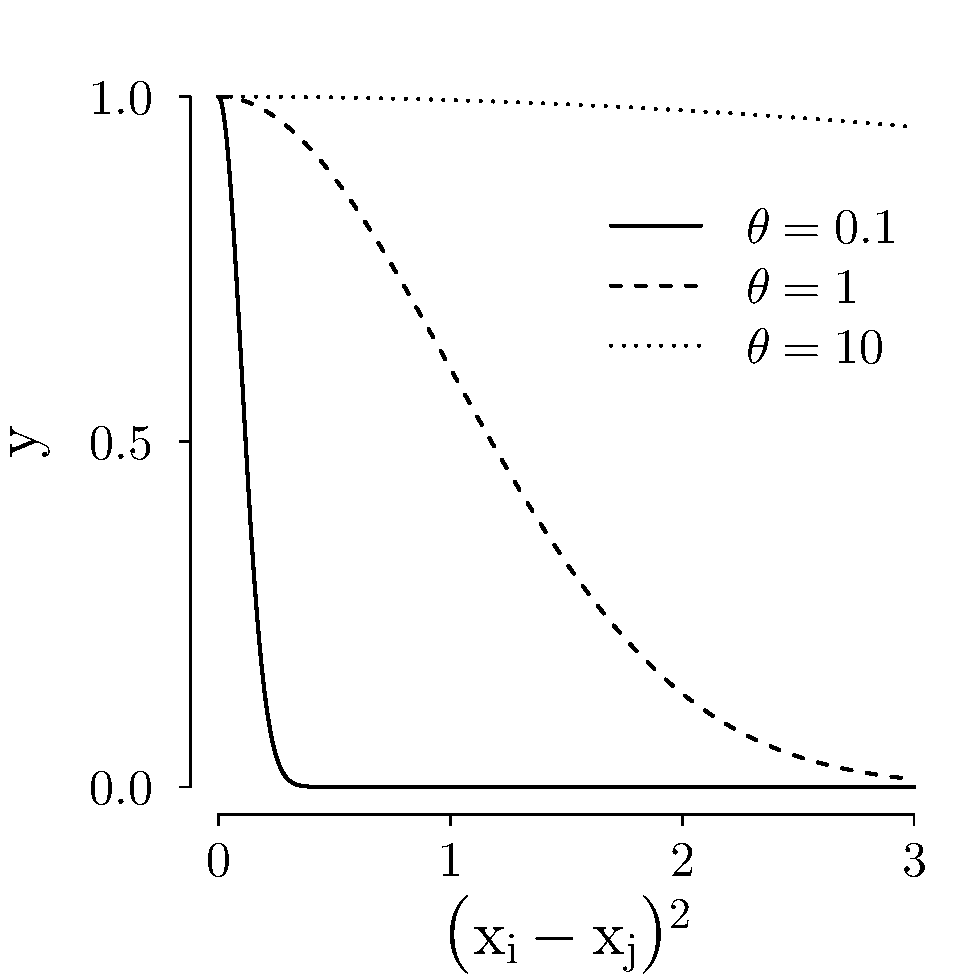
\includegraphics[scale=0.35]{../figures/chapter4/figures/plotCorrFunGauss.pdf}
	\caption[Gaussian correlation kernels with 3 different characteristic length scales]{Examples of Gaussian correlation kernels with 3 different characteristic length scales}
	\label{fig:plot_corrfun_gauss}
\end{figure}

The range parameter of a Gaussian kernel determines the range over which the distance between two input locations affects the output correlation.
To be precise, the notion of how similar (or dissimilar) two input locations are is defined relative to the characteristic length-scale.
With a very short range, the output of random functions becomes easily uncorrelated except for a very close (similar) inputs.
The realization of the process, therefore, will exhibit more erratic behavior in short range as it allows for more abrupt changes over shorter distance and less dependent of the neighboring values.
On the other hand, with a longer range, the output of random function tends to be highly correlated except for very different input values and thus the realization will exhibit more rigid pattern.
Gaussian kernel, however, always produces smooth realization.
That is, two input points that have a zero separation on are both continuous and differentiable (see the neighborhood of the origin of Fig.~\ref{fig:plot_corrfun_gauss}).
The Gaussian kernel is widely applied in the metamodeling literature and almost become a default choice for the correlation kernel \cite{Kennedy2006},
though as mentioned in \cite{Rasmussen2006} the overly smooth process can result in either physically unrealistic or numerically difficult situations (i.e., the resulting variance-covariance matrix is ill-conditioned for poorly select design points).

Fig.~\ref{fig:plot_corrfun_gauss_realizations} shows a comparison between realizations of a \gls[hyper=false]{gp} using Gaussian kernel for three different range parameters.
The short range, illustrated on the left panel, allows for more sudden change in the output values while the long range on the right shows smoother (and rigid) pattern for the same input domain ($0.0 \leq x \leq 3.0$). 
Also notice that the realizations with the shorter range produces more local maxima and minima.
\bigtriplefigure[pos=tbhp,
								 mainlabel={fig:plot_corrfun_gauss_realizations},
			           maincaption={Examples of realizations from \gls[hyper=false]{gp} with Gaussian correlation kernel for $3$ different values of range parameter. The plotting range of the $y$-axis for each panel are set to $\pm \, 3 \times \sigma$. Each process has the same process variance, $\sigma^2 = 1.0$},
			           mainshortcaption={Realizations of random function drawn from \gls[hyper=false]{gp} with Gaussian kernel},%
			           leftopt={width=0.30\textwidth},
			           leftlabel={fig:plot_corrfun_gauss_realization_1},
			           leftcaption={},
			           midopt={width=0.30\textwidth},
			           midlabel={fig:plot_corrfun_gauss_realization_2},
			           midcaption={},
			           rightopt={width=0.30\textwidth},
			           rightlabel={fig:plot_corrfun_gauss_realization_3},
			           rightcaption={},
			           spacing={},
			           spacingtwo={}]
{../figures/chapter4/figures/plotCorrFunGaussRealization_1}
{../figures/chapter4/figures/plotCorrFunGaussRealization_2}
{../figures/chapter4/figures/plotCorrFunGaussRealization_3}

\subsubsection{Power-Exponential Kernel}

The Gaussian correlation kernel belongs to a wider class of $2$-parameter kernel function family called the \emph{power-exponential} kernel and is given by \cite{Roustant2012,Santner2003,Rasmussen2006},
\begin{equation}
	r(x_i, x_j; \theta, p) = \exp{\left[ - \left( \frac{|x_i - x_j|}{\theta} \right)^p \right]} \, \text{for} \, \theta > 0.0 \, \text{and} \, 0 < p \leq 2
\label{eq:powexp_kernel}
\end{equation}

The parameter $\theta$ remains the range parameter of the process, while the additional parameter $p$ is referred to as the shape parameter of the process.
\marginpar{shape parameter}
Specifically, the shape parameter $p$ determines the differentiability of the process at the origin \cite{Abrahamsen1997}.
Fig.~\ref{fig:plot_corrfun_powexp} shows the correlation value of power-exponential kernel with three different values of $p$ and $\theta$ as function of $L_1$ norm ($|\mathbf{x}_i - \mathbf{x}_j|$).
\bigtriplefigure[pos=tbhp,
								 mainlabel={fig:plot_corrfun_powexp},
			           maincaption={Examples of power exponential kernel functions for different values of shape parameter $p$ and range parameter $\theta$ as function of $L_1$ norm.},
			           mainshortcaption={Examples of power exponential kernel functions},%
			           leftopt={width=0.30\textwidth},
			           leftlabel={fig:plot_corrfun_powexp_1},
			           leftcaption={},
			           midopt={width=0.30\textwidth},
			           midlabel={fig:plot_corrfun_powexp_2},
			           midcaption={},
			           rightopt={width=0.30\textwidth},
			           rightlabel={fig:plot_corrfun_powexp_3},
			           rightcaption={},
			           spacing={},
			           spacingtwo={}]
{../figures/chapter4/figures/plotCorrFunPowExp_1}
{../figures/chapter4/figures/plotCorrFunPowExp_2}
{../figures/chapter4/figures/plotCorrFunPowExp_3}

Although, strictly speaking, only when $p = 2$ the power-exponential correlation is differentiable at the origin (thus guarantee the smoothness of the realization),
the shape parameter does dictate the apparent roughness of the sample path drawn from the process as illustrated in Fig.~\ref{fig:plot_corrfun_gauss_realizations} \cite{Rasmussen2006}.
\bigtriplefigure[pos=tbhp,
								 mainlabel={fig:plot_corrfun_powexp_realizations},
			           maincaption={Several realizations from \gls[hyper=false]{gp} with power-exponential kernel functions of different shape $p$ and scale $\theta$ parameters.},
			           mainshortcaption={Examples of power exponential kernel functions},%
			           leftopt={width=0.30\textwidth},
			           leftlabel={fig:plot_corrfun_powexp_realization_1},
			           leftcaption={},
			           midopt={width=0.30\textwidth},
			           midlabel={fig:plot_corrfun_powexp_realization_2},
			           midcaption={},
			           rightopt={width=0.30\textwidth},
			           rightlabel={fig:plot_corrfun_powexp_realization_3},
			           rightcaption={},
			           spacing={},
			           spacingtwo={}]
{../figures/chapter4/figures/plotCorrFunPowExpRealizations_1}
{../figures/chapter4/figures/plotCorrFunPowExpRealizations_2}
{../figures/chapter4/figures/plotCorrFunPowExpRealizations_3}

It is argued in \cite{Marrel2008} that the power-exponential kernel function is an appropriate choice in metamodeling application due to its flexibility of representing different shape with respect to its regularity and differentiability mainly controlled through the additional parameter $p$.
\marginpar{exponential kernel}
For instance, Gaussian correlation kernel is a special case of the power-exponential kernel when $p$ equals to 2. 
Another special case is when $p = 1$ which is called the \emph{exponential} kernel.
In this particular case, realizations of which are depicted in Fig.~\ref{fig:plot_corrfun_powexp_realization_2}, the process is continuous but not differentiable \cite{Rasmussen2006}.

\subsubsection{Mat\'ern Class Kernel}

The Mat\'ern class correlation kernel is another $2$-parameter kernel family and it is given by the following formula \cite{Santner2003,Rasmussen2006}
\begin{equation}
	r(x_i, x_j; \theta, \nu) = \frac{2^{1-\nu}}{\Gamma(\nu)} \left(\frac{2\sqrt{\nu} |x_i - x_j|}{\theta}\right)^\nu K_{\nu}\left(\frac{2\sqrt{\nu} |x_i - x_j|}{\theta}\right)
\label{eq:matern_kernel}
\end{equation}
where positive $\nu$ and $\theta$ are the correlation kernel parameters;
$\Gamma(\circ)$ is the Gamma function;
and $K_\nu (\circ)$ is the modified Bessel function of order $\nu$.
In the literature, the value of $\nu$ is often restricted to half integer $\nu = n + \frac{1}{2}; n \in {0,1,\cdots}$,
because in that case the resulting modified Bessel function can be written simply as a finite series given by
\begin{equation}
	K_\nu(t) = \exp{-t} \sqrt{\frac{\pi}{2t}} \sum_{k = 0}^{n} \frac{(n+k)!}{k! (n-k)} \frac{1}{(2t)^k}
\label{eq:modified_bessel}
\end{equation}

The Mat\'ern class is considered more flexible than the power-expo\-nential kernel because the \emph{shape} parameter $\nu$ directly controls the number of differentiability of the process \cite{Stein1989}\footnote{that was not the case for power-exponential kernel because, strictly speaking, the process in only differentiable at $p = 2$ (and in fact, infinitely differentiable).}.
\marginpar{shape parameter $\nu$}
However, it was argued in \cite{Rasmussen2006}, that for machine learning application (i.e., regression and classification) only $\nu = 3/2$ (once differentiable) and $\nu = 5/2$ (twice differentiable) are of practical interest.
This is due to the fact that for $\nu < 3/2$ the process becomes too rough\footnote{in fact, it reduces to the exponential correlation function},
while for $\nu \geq 7/2$ the smoothness of the process realization cannot be distinguished anymore from an even smoother process.
These two Mat\'ern correlation kernels are given below \cite{Roustant2012,Rasmussen2006}
\begin{equation}
	r_{\nu=3/2}(x_i, x_j;\theta) = \left(1 + \frac{\sqrt{3}|x_i - x_j|}{\theta}\right) \exp{\left[-\frac{\sqrt{3} |x_i - x_j|}{\theta}\right]}
\label{eq:matern3_2}
\end{equation}
\begin{equation}
	r_{\nu=5/2}(x_i, x_j;\theta) = \left(1 + \frac{\sqrt{5}|x_i - x_j|}{\theta} + \frac{5|x_i - x_j|^2}{3\theta^2}\right) \exp{\left[-\frac{\sqrt{5} |x_i - x_j|}{\theta}\right]}
\label{eq:matern5_2}
\end{equation}

As the two previous kernels, the parameter $\theta$ serves as the range parameter of the process.
Example plots of the Mat\'ern kernel with different shape and range parameters are shown in Fig.~\ref{fig:plot_corrfun_matern}.
\normdoublefigure[pos=tbhp,
                  mainlabel={fig:plot_corrfun_matern},
                  maincaption={Mat\'ern kernels for $2$ different range parameters $\theta$ and, for each, $2$ different shape parameters $\nu$.},%
									mainshortcaption={Examples of Mat\'ern kernel functions},
                  leftopt={width=0.45\textwidth},%width=0.45\textwidth},
                  leftlabel={fig:plot_corrfun_matern_1},
                  leftcaption={},
                  %leftshortcaption={},%
                  rightopt={width=0.45\textwidth},%width=0.45\textwidth},
                  rightlabel={fig:plot_corrfun_matern_2},
                  rightcaption={},
                  %rightshortcaption={},
                  %spacing={\hfill}
                 ]
{../figures/chapter4/figures/plotCorrFunMatern_1.pdf}
{../figures/chapter4/figures/plotCorrFunMatern_2.pdf}

Examples realizations drawn from \glspl[hyper=false]{gp} with Mat\'ern kernel with different shape and range parameters are shown in Fig.~\ref{fig:plot_corrfun_matern_realizations}.
As expected, the realizations from Mat\'ern kernel with $\nu = 5/2$ is smoother than the ones from $\nu = 3/2$.
\normdoublefigure[pos=tbhp,
                  mainlabel={fig:plot_corrfun_matern_realizations},
                  maincaption={Example of sample paths drawn from \glspl[hyper=false]{gp} with Mat\'ern kernel for different range and shape parameters. One realization is drawn from each combination of the parameters.},%
									mainshortcaption={Sample paths drawn from \glspl[hyper=false]{gp} with Mat\'ern kernel functions},
                  leftopt={width=0.45\textwidth},%width=0.45\textwidth},
                  leftlabel={fig:plot_corrfun_matern_realizations_1},
                  leftcaption={},
                  %leftshortcaption={},%
                  rightopt={width=0.45\textwidth},%width=0.45\textwidth},
                  rightlabel={fig:plot_corrfun_matern_realizations_2},
                  rightcaption={},
                  %rightshortcaption={},
                  %spacing={\hfill}
                 ]
{../figures/chapter4/figures/plotCorrFunMaternRealizations_1.pdf}
{../figures/chapter4/figures/plotCorrFunMaternRealizations_2.pdf}

\subsection{Multidimensional Construction}

In order to create a valid multidimensional correlation kernel function from a valid $1$-dimensional correlation function given above, 
a tensor product construction is used as follows,
\marginpar{tensor product}
\begin{equation}
	R(\mathbf{x}_i, \mathbf{x}_j) = \prod_{d = 1}^{D} r_d \left(x_i^{(d)}, x_j^{(d)}\right)
\label{eq:tensor_product}
\end{equation}
where $r_d$ is a $1$-dimensional correlation kernel function for the $d$-th input dimension;
while $x_i^{(d)}$ and $x_j^{(d)}$ are a pair of values in the $d$-th input dimension.

Although it is possible to mix different types of correlation function or use different kind of multidimensional construction (see for example \cite{Higdon2002}),
the tensor product with the same correlation function for each input dimension is the most well-established 
and, by far, the most popular approach in the applied metamodeling literature to date \cite{Roustant2012,Sacks1989,Sacks1989a,Santner2003,Currin1991,Marrel2008,Bachoc2014,Kennedy2006,Jones2009}.

Fig.~\ref{fig:random_surfaces} shows two examples of realizations of random surface drawn from a multidimensional \gls[hyper=false]{gp} with the same process variance ($\sigma^2 = 10.0$) but with two different correlation kernels.
On the left is an example of a realization drawn from the \gls[hyper=false]{gp} using two Gaussian correlation kernel functions in which the characteristic length scale in the $y$-direction is four times the scale in then $x$-direction.
On the right is an example of a realization drawn from the \gls[hyper=false]{gp} using Mat\'ern correlation kernel functions.
For this case, the shape parameter is three times larger in the $x$-direction than in the $y$-direction.
As such, for both cases, the surface appears less smooth in one of the direction.
\bigdoublefigure[pos=tbhp,
                 mainlabel={fig:random_surfaces},
								 mainshortcaption={Random surface realizations},
                 maincaption={Two random surfaces drawn from two different multidimensional \gls[hyper=false]{gp} with the same process variance of $\sigma^2 = 9.0$. Differences in the scale (for Gaussian) and shape (for Mat\'ern) parameters for the inputs yield smoother path in one direction. The color scheme is the same for both plots with the range of $\pm \, 3 \times \sigma$.},
                 leftopt={width=0.475\textwidth},
                 leftlabel={fig:random_surface_gaussian},
                 leftcaption={Gaussian, $\theta_x = 0.5, \theta_y = 2.0$},
                 rightopt={width=0.475\textwidth},
                 rightlabel={fig:random_surface_matern},
                 rightcaption={Mat\'ern $\nu = 5/2$, $\theta_x = 1.5, \theta_y = 0.5$},
                 ]
{../figures/chapter4/figures/plotRandomSurface_1}
{../figures/chapter4/figures/plotRandomSurface_2}

%----------------------------
\subsection{Process Variance}
%----------------------------

For stationary \gls[hyper=false]{gp}, the shape of the sample path is determined solely by the form of the correlation.
The role of the process variance according to Eq.~(\ref{eq:cov_function}) is to determine the scale of the magnitude of the output variation. 
Fig.~\ref{fig:plot_process_variance} gives an illustration of the realizations drawn from a set of \glspl[hyper=false]{gp} with the same kernel correlation function (i.e., Gaussian kernel with $\theta = 1.0$), 
but with different values of process variance.
As it can be seen, the visible features of the realizations remain very similar to each other.
What has changed, however, is the scale of the variation in the output space.  
\bigtriplefigure[pos=tbhp,
								 mainlabel={fig:plot_process_variance},
			           maincaption={Realizations of \gls[hyper=false]{gp} with Gaussian correlation kernel for $3$ different values of process variance. The plotting range of the $y$-axis for each panel is set to $\pm \, 3 \times \sigma$.},
			           mainshortcaption={Effect of different process variance values on GP realization},%
			           leftopt={width=0.30\textwidth},
			           leftlabel={fig:plot_process_variance_1},
			           leftcaption={},
			           midopt={width=0.30\textwidth},
			           midlabel={fig:plot_process_variance_2},
			           midcaption={},
			           rightopt={width=0.30\textwidth},
			           rightlabel={fig:plot_process_variance_3},
			           rightcaption={},
			           spacing={},
			           spacingtwo={}]
{../figures/chapter4/figures/plotProcessVariance_1}
{../figures/chapter4/figures/plotProcessVariance_2}
{../figures/chapter4/figures/plotProcessVariance_3}

%-----------------------------------------------------
\subsection{Mean Function}\label{sub:gp_mean_function}
%-----------------------------------------------------

Mean function is the drift term in the \gls[hyper=false]{gp} model.
Strictly speaking, incorporating other than a constant mean function to the specification of a \gls[hyper=false]{gp} introduces non-stationarity to the process.
But as the known mean function can always be removed from the formulation (i.e., by \emph{centering}), the process, especially with respect to its correlation function, can still be considered stationary.
Fig.~\ref{fig:plot_mean_function_unconditional} shows several realizations drawn from $3$ \glspl[hyper=false]{gp} having the same covariance kernel, but with three different mean functions.
As it can be seen, the process are centered differently for the $3$ \glspl[hyper=false]{gp}. 
The choice of the mean function determines the behavior of the conditional process (where it is constrained by the observed data) in the region far away from the available data.
\bigtriplefigure[pos=tbhp,
								 mainlabel={fig:plot_mean_function_unconditional},
			           maincaption={The effect of using three different mean functions (in dashed lines) on the realization of \gls[hyper=false]{gp} having the same covariance kernel (Gaussian). The scales in the axes are arbitrary.},
			           mainshortcaption={Effect of different mean functions on GP realization having the same covariance kernel},%
			           leftopt={width=0.30\textwidth},
			           leftlabel={fig:plot_mean_function_unconditional_1},
			           leftcaption={constant},
			           midopt={width=0.30\textwidth},
			           midlabel={fig:plot_mean_function_unconditional_2},
			           midcaption={linear},
			           rightopt={width=0.30\textwidth},
			           rightlabel={fig:plot_mean_function_unconditional_3},
			           rightcaption={quadratic},
			           spacing={},
			           spacingtwo={}]
{../figures/chapter4/figures/plotMeanFunctionUnconditional_1}
{../figures/chapter4/figures/plotMeanFunctionUnconditional_2}
{../figures/chapter4/figures/plotMeanFunctionUnconditional_3}

The use of the mean function provides an opportunity to incorporate prior knowledge of the process before observing any data or to improve the resulting model performance for extrapolation purpose \cite{Ginsbourger2009,Roberts2012}.
However, without a very specific knowledge of how a process is expected to behave, it is difficult to completely specify a justifiable mean a priori.
Indeed, it was argued in \cite{Currin1991} that the use of either zero or constant mean in GP to model a process signifies a vague or the least informative prior to the unknown.
This eventually leads to the most generic formulation.